\chapter{Lightweight reasoning for student models.}

If all students would take the same linear learning path, then we could represent student progress by a number.
For example, if Mary is working on exercise 6 and Fred on exercise 5, then she is one exercise ahead.
Adaptivity to individual needs is a key feature that distinguishes an \gls{its} from other forms of computer aided instruction.
Students may take different routes through the material, depending on individual needs and preferences.
After exercise 3 the \gls{its} may have given the students the option to choose from exercise 4, 5 and 6.
And now we cannot say that Mary is ahead of Fred, but only that both have completed exercise 3.

To measure student progress in an \gls{its} we can use partial orderings.
Partial orderings are very common in learning materials. 
Many authors indicate alternative routes to read chapters based on individual interests.

This chapter describes  how lattices can be used to reason about student progress (Section \ref{stmlat}).
The structure of the student model is described in Section \ref{sec:stmedum}.
Section \ref{sec:lwrules} describes the rule system in general, and Section \ref{sec:rllearntask} shows how this can be applied in the \gls{tensteps}.


\section{Student model as a lattice.}
\label{stmlat}

\subsection{Progress indicators and progress vectors}
An overlay model is the most popular form of student model \citep{chrysafiadi_2013}.
It is in the simplest form a list of domain concepts.
For each concept a value is assigned as an indication of student progress.

\begin{definition}
A progress indicator is a value that ranges over a lattice with a bottom.
\end{definition}
\begin{definition}
A progress vector is a set of items. Each item is a (name, value) pair, where the value is a progress indicator.
\end{definition}

In Section \ref{sec:lattices} we have seen that lattices may be combined as tuples to form a new lattice.
Thus it follows that a tuple of progress indicators is also a progress vector, and that tuples may be nested to any depth.

In a student model we must keep a large number of progress indicators, and tuples are not practical.
Instead of using a number for each dimension we define a set of names $\{name_{1}, name_{2}, ... ,name_{n}\}$. 
A tuple of progress indicators $(pi_{1}, pi_{2}, ..., pi_{n})$ corresponds to a progress vector
$\{(name_{1}, pi_{1}), (name_{2}, pi_{2}), ... , (name_{n}, pi_{n})\}$.

It is not necessary to store all values,  an item is assumed to have a value of bottom if not present.
The canonical form is to leave out elements at bottom value. 

Progress vectors have a one to one correspondence to tuples.
The join, meet, bottom and $\leq$ are defined for progress vectors in the same way as for the corresponding tuples.
Thus a progress vector is a notational convention for the application of lattices in a student model.

Progress vectors form a lattice with a bottom value, and can be used as progress indicators.
This makes the definition recursive.
Progress vectors can be nested to any depth. 

\begin{definition}
Atomic progress indicators are progress indicators that can not be decomposed. 
\end{definition}

So our model is made up of atomic progress indicators combined as progress vectors.
In Section \ref{apival} we discuss atomic progress indicators.

\subsection{Atomic progress indicators in the student model.}
\label{apival}
The dividers of 60 may be an interesting example of the lattice structure, but we will not further use lcm and gcd.
In this thesis we work with three types of atomic progress indicators, although many others are possible.


\begin{description}
\item [Boolean values] ($PiBool$)\hfill \\
Boolean values can be used to indicate that the student masters a concept or an exercise is completed.
Boolean values form a lattice, when we take disjunction as join and conjunction as meet operation.
Lattices have duality properties, so we could turn this around, but to avoid confusion we will not do so.
\item[Counters]  ($PiCount$) \hfill \\
Counters are positive integral numbers. Counters form a lattice. We take zero as bottom value, max for join and min for meet.
It has a linear ordering, which is a stronger form of ordering than partial ordering.

A special operation is needed to increment or add counters. 
For this purpose we have added an operator $\addjoin$. 
For counters it adds the counter. For any other progress indicator it is equivalent to join.
If we update the student model with this operator, it is still monotonously increasing.


\item[Knowledge level] ($PiBloom$)  \hfill \\
We need indicators for the levels of learning of domain concepts.
Bloom defined a taxonomy with hierarchical levels of learning. This is still used today \citep{BHALERAO201756}.
The Bloom taxonomy forms  a set with  linear ordering:\\
\{Knowledge, Comprehension, Application, Analysis, Synthesis, Evaluation\}.\\
We use this as an enumeration to which we add ``Ignorant'', and use this as the bottom value. 

\end{description}

We must mention that the TenSteps aims at the development of integrated skills.
The Bloom metric is somewhat one-sided in that is aims only at the cognitive domain.  

\subsubsection{Other possible progress indicators}
\label{sec:atomicpi}

Any datatype that forms a lattice with a bottom value can be used as progress indicator.
Booleans, enumerated datatypes or ranges of integers are acceptable as progress indicators.
Real values in the interval [0, 1] form a lattice with min and max, and can be used as probabilities.

In Figure \ref{fig:progressIndicators} we see a set of values that form a partially ordered set with a bottom value (A).
This may be a state model $\mathit{PiState = \{A, \; B, \; C, \; D, \; E, \; F, \; G\}}$.  
It is not a complete lattice. We can see that for example $C \sqcup D = E$ and $E \sqcap G = A$.
We can not join any two elements: e.g. $E \sqcup G$ and $B \sqcup F$ are undefined. 
 
 


\begin{Figure}
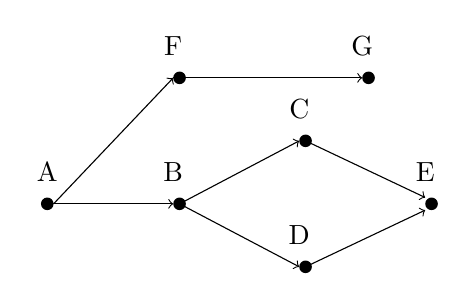
\begin{tikzpicture}[scale=0.08]

\fill[black] (10,20) circle(1);
\node (o3) at (10,25) {A};

\draw [->] (10,20) -- (30,20);
\fill[black] (31 ,20) circle(1);
\node (o3) at (30,25) {B};

\draw [->] (31,20) -- (50,30);
\fill[black] (51 ,30) circle(1);
\node (o3) at (50,35) {C};

\draw [->] (31,20) -- (50,10);
\fill[black] (51 ,10) circle(1);
\node (o3) at (50,15) {D};

\draw [->] (51,10) -- (70,19);
\fill[black] (71 ,20) circle(1);
\node (o3) at (70,25) {E};

\draw [->] (51,30) -- (70,21);

\draw [->] (11,20) -- (30,40);
\fill[black] (31 ,40) circle(1);
\node (o3) at (30,45) {F};

\draw [->] (30,40) -- (60,40);
\fill[black] (61 ,40) circle(1);
\node (o3) at (60,45) {G};



\end{tikzpicture}
\caption{Progress indicators poset PiState}\label{fig:progressIndicators}
\end{Figure}

This can be used as progress indicator in the following ways:
\begin{itemize}
\item We could add an artificial extra element T following G and E, such that $ G \sqcup E = T$.
\item We can accept the fact that we have a model constraint and throw an exception when an impossible join (e.g. $F \sqcup C$) is attempted.
\item A value from PiState can be represented as a tuple: $\{(v1,v2) \mid v1 \in \{A, F, G\} , v2 \in \{ A,B,C,D,E\}\} $ for each path. 
In this case we also have a model constraint  that either $v1$ or $v2$ is bottom.
Thus $(A,A)$,  $(A,D)$, $(G, A)$ are valid, but $(F,B)$ is an invalid state. 
\item Another solution is to use boolean indicators to represent the state.
The indicators become true as the model reaches greater values.
In that case there are many constraints, for example,  if C is true then A and B may be True, but D, F and G must not be true.
\end{itemize}
Only the first solution conforms completely to our definition of progress indicators.
But from a software engineering point of view it makes little difference.
In the first case we get a model constraint that values may not assume the value T.

We update the student model with a join operation, so once the student is on path F he cannot reach E anymore.
This does not have to be a problem, for example if it is an end state when an exercise is finished.

\subsubsection{Some examples with atomic progress indicators}

We allready mentioned that an important property of lattices is that they can be combined, to form another lattice.
The tuples $(v1, v2, v3) \in PiBool \times PiCounter \times PiBloom$ form a lattice.
For example:
\begin{itemize}
\item $\mathit{bottom} =  (\mathit{False}, 0, \mathit{Ignorant})$
\item $ (\mathit{False}, 4, \mathit{Analysis})  \sqcup (\mathit{True}, 5, \mathit{Comprehension}) = (\mathit{True}, 5, \mathit{Analysis})$
\item $ (\mathit{False}, 4, \mathit{Analysis})  \sqcap (\mathit{True}, 5, \mathit{Comprehension}) = (\mathit{False}, 4,  \mathit{Comprehension})$
\item $(\mathit{False}, 3, \mathit{Comprehension}) \leq (\mathit{True} , 5, \mathit{Analysis}) = \mathit{True}$
\item $ \mathit{comparable}\; \; (\mathit{False}, 4, \mathit{Analysis})\; \;  (\mathit{True}, 5, \mathit{Comprehension}) = \mathit{False}$
\end{itemize}


\subsection{Progress vectors for a student model}
\label{pv4sm}

In step four of the  \gls{tensteps} a domain model is developed,  that describes the knowledge domain.
Knowledge domains may contain concepts and terminology, structures and causal relationships.
In the domain of functional programming the syntax and prelude functions have a certain structure.
Mechanisms such as strict and lazy evaluation are causal relationships.   

An overlay model uses a set of elements that cover the knowledge domain.
In the simplest form a boolean value is assigned to each element \citep{brusilovskiy_1993}.
We use progress indicators in our student model. 
Our student model is an overlay model in the form a progress vector.
The student model may contain elements from the domain model, as well as indicators of exercise progress.


In  table \ref{student.progressvec1} we see (part of) a progress vector with student progress.
We have indicated the type of each atomic indicator.

\begin{table}[H]
\begin{tabular}{| l | l | l |}
\hline
Key & Progress indicator value & type\\
\hline
DM.Recursion & Knowledge & PiBloom \\
CAUS.SimpleExpressionEvaluation & Application & PiBloom\\
SYN.IFexpression & Knowledge  & PiBloom\\
PRE.GTR & Knowledge  &PiBloom\\
PRE.Plus & Comprehension  & PiBloom\\
RL.expr.plus& 1 & PiCount\\
CS.double& True & PiBool\\
\hline
\end{tabular}
\caption{Example of a progress vector for an overlay student model.}
\label{student.progressvec1}
\end{table}
 
In practice this might well contain hundred or more items.
The table contains indicators for knowledge levels for domain concepts.
This student has read materials on recursion, and he can evaluate simple expression.
He applied a rule expr.plus once and he has successfully completed an exercise of type double.
The value type should be obvious: True for PiBool, Comprehension is PiBloom and numbers are counters.

\subsubsection{Naming conventions}
As table \ref{student.progressvec1} shows, we have applied a naming convention using prefixes for different kind of indicators.

\begin{table}[H]
\begin{tabular}{| l | l | l |}
\hline
Prefix & Used for\\
\hline
TC & Task class\\
LT & Learning task (exercise)\\
ES & Educational indicators \\
EX & Exercise type \\ 
RL & Rewrite rules\\
DR & Domain reasoner\\
PRE & Prelude \\
DM & Domain concepts \\
SYN & Syntax\\
\hline
\end{tabular}
\caption{Prefixes used in naming convention.}
\label{student.namingConvention}
\end{table}

Table \ref{student.namingConvention} shows the prefixes we use.
We will work with deeply nested vectors.
We use slashes to indicate the pathname of a nested  value or vector in the model, similar as for filenames.
The student model has an absolute position of \\
\indent ``$\mathit{/ES.student}$``.\\
An absolute pathname for an exercise in a task class might be: \\
\indent``$\mathit{/TC.01.ExpressionEvaluation/LT.01.double}$''.\\
We often use the term exercise instead of learning task. 
In rules we use variables that range over exercise positions, these are written as $\$exercise$. 

Many traditional \glspl{its} separate student knowledge, educational progress and misconceptions \citep{brusilovskiy_1993}, but we use just one vector.
Any author is free to choose a different structure and naming conventions.
 



\subsubsection{Updating the student model}


An item corresponds to a domain concept or progress with exercises and task classes.

The successful completion of an exercise provides evidence of a certain level of mastery of some concepts that form a progress vector.
If we denote the student model after exercises $n$ as $SM{_n}$ and the progress vector as $e{_n}$, then we can update the student model:
\begin{equation} \label{smupdate}
SM_{n} = SM_{n-1} \sqcup   e{_n}
\end{equation} 
Equation \ref{smupdate} makes the student model a monotonous function of $n$:
\begin{equation} 
SM_{n-1} \leq SM_{n} 
\end{equation} 
We have required that progress indicators have a bottom value and this make it easy to start with:
\begin{equation} 
SM_{0} = \bot 
\end{equation} 
A top value is not needed, as some progress indicators have a range wider then required.
We may not have material in the \gls{its} to reach the level ''Evaluation'' for every topic. 
We will be satisfied if the student executes a rule two or three times, however, our counters can easily count up to a million.




\section{Student model and educational model}
\label{sec:stmedum}
A traditional architecture for an \gls{its} consists of a student model and an educational model as separate services.
The services might be implemented in separate web or REST services.
A separation of concerns is definitely a good idea.

In this thesis, however, we will put everything together in one variable of the type progress vector.
We will refer to this as the model.
The model has a hierarchical structure as shown in Figure \ref{model.hier}.
\begin{Figure}
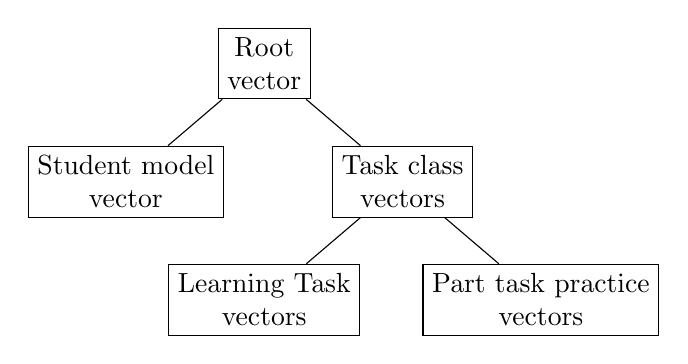
\begin{tikzpicture}[sibling distance=10em,
  every node/.style = {shape=rectangle, 
    draw, align=center}]]
  \node {Root \\vector}
    child { node {Student model \\vector} }
    child { node {Task class \\vectors}
      child { node {Learning Task \\vectors} }
      child { node {Part task practice \\vectors} } };
\end{tikzpicture}
\caption{Hierarchical structure of model components}
\label{model.hier}
\end{Figure}

The left branch contains the student model as discussed in Section \ref{pv4sm}.
The model contains the progress of only one student.
The right branch is the educational model, which is decomposed in multiple task classes.
Each task class contains multiple learning tasks and part-task practices.
This is modelled after the blueprints from the \gls{tensteps}.

The whole tree is build up from nested progress vectors.
From now on we will often prefix vector by their usage.
The root vector is the root of the structure.
It contains the vector for the student model, the task class vectors, which contain learning task vectors and part task practice vectors.

The root vector is a progress indicator and can be joined and compared with similar shaped structures.
A step vector is such a structure, used to update the model after each task step.
A step vector is derived from a request-response cycle with the diagnose service from a domain reasoner.

The step vector has the same structure as shown in Figure \ref{model.hier}.
A step vector might theoretically contain a student root vector to update the student model directly. 
In the scenarios we use step vectors with a task class vector and a learning task vector with subvectors.
We use rules that evaluate the exercise vector to update the student model vector.

We use an add ($\addjoin$) operation to update the model, to be able to count strategy and rule executions.
Step vectors may also result from other interactions e.g. multiple choice questions.

Similar like the student model, the whole model is updated with join operations and therefore monotonically increasing.
The model mixes progress information with metadata, such as objectives and prerequisites.
It is possible to have variations in metadata per student.
For example certain students may benefit from doing more exercises than others.

Another alternative way to look at the model is as an ontology model.
The student and the educational components can be seen as individuals in an ontology model.
These individuals have relationships and data properties that are here implemented in the structure of the progress vector.
This model can be queried and inferences about student progress can be made by a rule system.

\subsection{Contents of a learning task vector}
\label{sec:rllearntask}



\begin{table}[H]
\begin{tabular}{| l | l | l |}
\hline
Name & Type& Description \\
\hline
DR.Rules & Vector & Rewrite rule executions\\
ES.successCriteria & Vector &  Minimum rule executions\\
ES.objective & Vector & Objectives of task\\
ES.prerequisite & Vector &  Prerequisites of the task\\
DR.created & PiBool & The exercise is started  \\
ES.finished & PiBool & The exercise is finished \\
ES.success & PiBool & The exercise is finished successfully\\
ES.failure &PiBool & The student did not complete the exercise \\
ES.error &PiBool &  The student made errors during the exercise\\
\hline
\end{tabular}
\caption{Subcontent of a learning task vector.}
\label{student.progressvec2}
\end{table}

Table \ref{student.progressvec2} details the content of a learning task vector.
The first two elements are related. A step vector updates DR.Rules on each rule execution.
The ES.successCriteria is set up by the author and defines the minimum number of rule executions.
So if $\mathit{DR.Rules \geq ES.successCriteria }$ he did execute the rules expected, or otherwise he may have asked hints.

The prerequisites and objectives can be compared or joined with the student model.
If $\mathit{ES.student \geq ES.prerequisite}$ then the student meets the prerequisites (ES.student denotes the student model vector). 
If $\mathit{ES.student \geq ES.objective}$ then the exercise may be too easy.

The booleans indicate the state of the exercise. The DR. created is set by a step vector when the exercise is started.
The other flags are inferred by rules depending on how the exercise was completed. The rules will be discussed later.




\section{Lightweight inferencing with rules}
\label{sec:lwrules}
It is not enough to add up counters of rule executions to update the student knowledge.
Some intelligent technology, a rule system in this case, is used to infer updates to the student model.
\subsubsection{Rule structure}
\label{sec:rulestruc}

The rule system that we propose to reason about the student model works similar to other rule systems.
A rule has  the following form:
\begin{equation} \label{rl}
p{_1}, . . , p{_n} \rightarrow c{_1}, . . , c{_m}
\end{equation} 
The $p{_1}, . . , p{_n}$ are a set of predicates and the $c{_1}, . . , c{_m}$ are conclusions.
A predicate has variables that range over the individuals in the ontology.
We write commas between the predicates, when the rule is executed the predicates are evaluated and combined with a logical conjunction.
When all predicates evaluate to $\mathit{True}$, the rule fires. 

The conclusions are progress vectors in the shape of the model.
One rule may have multiple conclusions. The conclusions from all rules that fire are joined into a single conclusion.
Often a part of the model is copied somewhere else to form a conclusion.
For example, when an exercise is completed successfully we join the exercise objectives to the student model.
In our system we have bottom as a zero-element, so if some predicate fails we can say that we conclude bottom.


Some examples of predicates are the following:
\begin{itemize}

\item $\mathit{isTaskClass(?tc), \; isLearningTask(?lt), \; isStudent(?st)}$\\
Individual $\mathit{tc}$ is a task class $\mathit{and}$  $\mathit{st}$ is the student $\mathit{and}$ $\mathit{lt}$ a learningtask.
The question marks denote the variables for individuals (after SWRL/OWL). 
The individuals range over the the whole ontology; this way we make a selection, in fact a cross product of three subsets.
These are examples of unary predicates.  

\item $\mathit{belongsTo(?lt, ?tc)}$\\
An example of a binary predicate indicating we only want learningtasks that belong to the task class.

\item  $\mathit{ isLearningTask(?lt), \; prerequisites(?lt, ?pre),  \; ?st \; \geq \; ?pre}$ \\
The item $\mathit{lt}$ is a learningtask  $\mathit{and}$  $\mathit{lt}$ has prerequisites $\mathit{pre}$  $\mathit{and}$ some item  $\mathit{st}$ is greater then  $\mathit{pre}$.
If  $\mathit{st}$ is a student model, then the student meets the prerequisites of $\mathit{lt}$, as described in section \ref{sec:rllearntask}. 

\item $\mathit{isLearningTask(?lt), \; exerciseprogress(?lt, ?ep), \; succescriteria(?lt, ?sc), \; ?ep \geq ?sc }$\\
The learning task $\mathit{lt}$ has made a progress of $\mathit{ep}$ and success criteria $\mathit{sc}$.
The exercise is completed successfully, as $\mathit{?ep \geq ?sc}$. 
\end{itemize}

These predicates may be used in rules, but it is also possible to query the model with predicates, for example to select exercises.


\subsection{The loop and rule implementation in Haskell}
Rule systems as well as databases have advanced mechanisms to work efficiently.
Having multiple nested loops ranging over all individuals is expensive.
When assertions are added to the ontology, this may enable other rules to fire and require an extra run.

In other rule systems users may be required to prioritise rules as rules may influence each other.
OWL/SWRL is designed such that the rules can be run until a fixpoint is reached.
This creates restrictions, for example, we cannot update or delete assertions.
The rules are monotone in the sense that they only add facts.

In Haskell we do not have an advanced completely generic rule engine.
It turns out that we can do most of the reasoning if we iterate over the task classes and learning tasks.
Each rule is called with a tuple of four parameters: (root, student, taskclass, learningtask).
The conclusions we derive are progress vectors with the same shape as the model. 
After the rules execute we join all conclusions to the model.
Because rules may affect each other we run this mechanisme a number of times until we reach a fixpoint.
All our individuals have the same underlying type of being a (Wrapped) progress vector.

This means:
\begin{itemize}
\item Predicates have type:\\
$\mathit{ RulePredicate :: (Root, Student, TaskClass, LearningTask) \rightarrow Boolean}$\\
During the iteration each predicate can be evaluated to a True or False value.
 
\item For conclusions we use the type DerivedFact:\\
$ \mathit{ DerivedFact :: (Root, Student, TaskClass, LearningTask) \rightarrow Root}$\\
A DerivedFact can be executed during the iteration to return a conclusion in the form of a progress vector.

\item $\mathit{Root, Student, TaskClass}$ and $\mathit{LearningTask}$ are (wrapped) progress vectors.

\item The predicates  $\mathit{isTaskClass(?tc), \; isLearningTask(?lt), \; isStudent(?st), \;belongsTo(?lt, ?tc)}$\ shown in section \ref{sec:rulestruc} are now implicit, due to the iteration.

	
\item To create rules we define an operator:\\ 
$ (\rulearrow) :: \mathit{[RulePredicate] \rightarrow [DerivedFact] \rightarrow Rule}$\\
These rules can be executed in the iteration, with the four parameters.
 
\end{itemize}

Our rule engine may be sensitive to rule execution order. 
There are some strategies that can be followed to prevent unwanted results.
 \begin{itemize}
\item Rules can be made once-only, e.g some value is set and a predicate prohibits firing the rule again.
\item Rules must specify predicates that are disjunct, so that in each case only one specific action takes place.
\end{itemize}

If a rule keeps deriving the same fact, it does not have to be a problem as the join operation absorbs the derived fact ($ a \sqcup a = a $).
The rules execute after the student model is updated with the progress vector derived from the domain reasoner response.
For some rules it may be necessary to run multiple times until a fixpoint is reached.

\section{Rules for exercises}

In this section we describe the rules used to implement guidelines from the \gls{tensteps}.



\subsection{Exercise states}

We have defined a specific progress indicator for exercise state, to keep track of which exercises have been attempted and the outcome.
The exercise state is not kept in a single variable, but inferred from the set of boolean indicators that we showed in table \ref{student.progressvec2}.
This works like the example we showed in Figure \ref{fig:progressIndicators}.
An exercise has the following state model:


\begin{Figure}
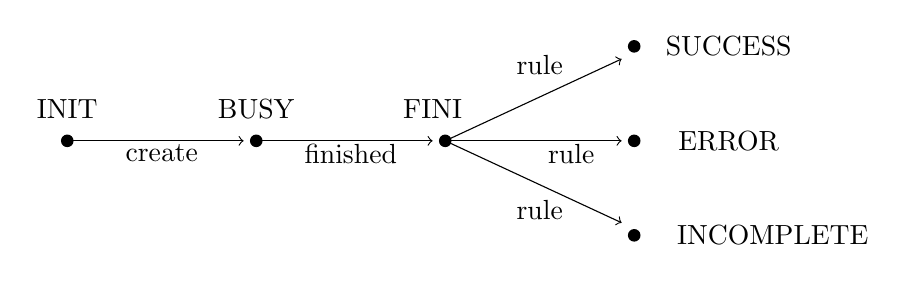
\begin{tikzpicture}[scale=0.08]

%\fill[black] (20,20) circle(1);
%\node (o3) at (20,25) {INIT};
\fill[black] (40,20) circle(1);
\node (o3) at (40,25) {INIT};
\fill[black] (70,20) circle(1);
\node (o3) at (70,25) {BUSY};
\fill[black] (100,20) circle(1);
\node (o3) at (98,25) {FINI};

\fill[black] (130,5) circle(1);
\node (o3) at (152,5) {INCOMPLETE};
\fill[black] (130,20) circle(1);
\node (o3) at (145,20) {ERROR};
\fill[black] (130,35) circle(1);
\node (o3) at (145,35) {SUCCESS};


\node (o3) at (55,18) {create};
\node (o3) at (85,18) {finished};
\node (o3) at (115,32) {rule};
\node (o3) at (120,18) {rule};
\node (o3) at (115,9) {rule};



%\draw [->] (20,20) -- (38,20);
%\draw [->] (20,20) -- (40,15);
%\draw [->] (40,15) -- (58,19);

\draw [->] (40,20) -- (68,20);
\draw [->] (70,20) -- (98,20);

\draw [->] (100,20) -- (128,7);
\draw [->] (100,20) -- (128,20);
\draw [->] (100,20) -- (128,33);


\end{tikzpicture}
\caption{Exercise state}\label{fig:ltstate}
\end{Figure}

Exercises start in state INIT. When an exercise is started, a create request is send to the domain reasoner.
This results in ``DR.created'' to be set in the exercise.
When an exercise is finished the domain reasoner sets a finished flag in the message, resulting in ES.finished being set.


We depend on some component (the user interface perhaps) to send us a finished message when the student stopped with the exercise.
The domain reasoner is stateless, and there is no formal exercise termination send to the domain reasoner.



\subsection{Rules for exercise completion}
\label{subs:rules}

A rule consists of a set of RulePredicates and a set of DerivedFacts.
When all RulePredicates evaluate to true for a given exercise and student knowledge, the DerivedFacts are evaluated to collect the conclusions. 

Conclusions have the same form as the model.
The first rule below, for example, creates a set indicators in the student part for each indicator in the objectives of the exercise.
Effectively it copies the contents of a vector to another place in the model.
The engine runs all DerivedFacts and joins the results together.

When an exercise is finished (state FINI) exactly one of four rules may fire:

\begin{description}
\item[Success rule]:\\ 
$\mathit{/\$exercise/FINI}$,\\
$\mathit{not\; /\$exercise/DR.rules/ES.error}$, \\
$\mathit{/\$exercise/DR.Buggy == bottom}$,\\
$\mathit{/\$exercise/DR.Rules \geq /\$exercise/ES.successCriteria}$ \\
$\rightarrow$\\
$\mathit{/\$exercise/ES.success}\;\mathit{True}$ (state becomes SUCCESS),\\
$\mathit{\{/ES.student/obj} \; | \; \mathit{obj \in /\$exercise/ES.objective}\}$.

\item[Incomplete rule]:\\ 
$\mathit{/\$exercise/FINI}$,\\
$\mathit{not\; /\$exercise/DR.rules/ES.error}$,\\
$\mathit{/\$exercise/DR.Buggy == bottom}$,\\
$\mathit{not\; /\$exercise/DR.Rule \geq /\$exercise/ES.successCriteria}$ \\
$\rightarrow$\\
$\mathit{ /\$exercise/ES.incomplete \; True}$  (state becomes INCOMPLETE).

\item[Error rule]:\\ 
$\mathit{/\$exercise/FINI}$,\\
$\mathit{/\$exercise/DR.Buggy == bottom}$,\\
$\mathit{/\$exercise/DR.rules/ES.error}$ \\
$\rightarrow$\\
$\mathit{/\$exercise/ES.error\; True}$  (state becomes ERROR).

\item[Buggy  rule]:\\ 
$\mathit{/\$exercise/FINI}$,\\
$\mathit{not \; /\$exercise/DR.Buggy == bottom}$\\
$\rightarrow$\\
$\mathit{\{/ES.student/bug} \; | \;\mathit{bug \in /\$exercise/DR.Buggy }\}$,\\
$\mathit{/\$exercise/ES.error\; True}$  (state becomes ERROR).

\end{description}

 
The success rule must calculate an update to the student model.
The rewrite rules that the student executes are counted in a vector with name DR.rules.
This is compared with the vector ES.successCriteria to determine successful completion.

The objectives of the exercise are joined to the student model. An exercise double might contain:\\
``$\mathit{/TC.01.ExpressionEvaluation/LT.01.double/ES.objective/EX.double\; True}$''.\\
The rule would move this objective to the student model:\\
``$\mathit{/ES.student/EX.double\; True}$''.\\
After all rules are executed the conclusions are joined to the model.

When the student made a miscalculation or another error,  the exercise may be completed.
After the exercise is finished, the Error rule fires and puts the exercise in state ERROR.
We do not update the student knowledge. 
The error rule just prevents any of the other rules to run again.

If the student took a shortcut, such as just giving the answer, or just gave up the exercise, it ends in the state INCOMPLETE.
Also when a hint is given or other procedural support given the exercise ends in INCOMPLETE.
In spite of the fact that the student may probably learn the most from his mistakes, we do not update the model after a procedural support or errors.

The \gls{tensteps} prescibes that the student may proceed to a higher task class when he can carry out exercises without requiring
procedural support. This is why we only update the student model after a successful exercise completion.

The buggy rule fires in case of a misconception. 
Domain reasoners may have buggy rewrite rules, that fire when certain errors are recognised.
For example, the student should have added a value, but subtracted it.
Buggy rewrites are administered in a separate vector DR.Buggy.
It is assumed that the exercise will be terminated in this case, so DR.Buggy will only contain one value.
We add this to the subvector of the student with bugs.
Queries  use this information to select an intervention, for example a part-task exercise.

  

\subsection{Fast students and Knowledge Space Theory.}
\label{sec:fststdntrule}
The Knowledge Space Theory (KST) is a psychometric theory, that is used for selection of assessment questions \citep{doignon_falmagne_2016}, \citep{TUGraza}.
A learning space is defined as a set of knowledge structures that form a partial ordering.
A knowledge structure is a subset of learning items that include all prerequisite items.
For example, the exercise types  from Section \ref{sec:drmaxidble} are double, maxi and combined. 
Exercise double is easier than maxi, which is easier than combined, therefore the recommended order is double, maxi, combined.
The sets ks1: \{double\}, ks2:\{double, maxi\} and ks3:\{double, maxi, combined\} are knowledge structures.
In a learning space the knowledge stuctures have an inner fringe of structures that have one item less, and an outer fringe with structures that have one item more.
For example in our task class, the inner fringe of ks2 is ks1 and outer fringe is ks3.

Suppose a students starts with an advanced exercise of type combined and completes it correctly.
It would make little sense to recommend the easier exercises double and maxi.

A rule can be defined to solve this issue.
The rule will add the prerequisites of completed exercises to the student model.
\begin{description}
\item[Fast student rule]:\\ 
$\mathit{/ES.student/ \geq /\$exercise/ES.objective}$ \\
$\rightarrow$\\
$\mathit{\{/ES.student/preq} \;| \; \mathit{preq \in /\$exercise/ES.prerequisite}\}$.
\end{description}

\subsection{Exercise recommendation query}
\label{sec:exrecquer}
After all facts have been derived, the model can be queried.
For example the user interface can display a list of exercises, that have been completed, with results, or display the student model.

Exercise selection is an important aspect in both \gls{its} and the \gls{tensteps}.
We may want to select exercises in the outer fringe of the knowledge space.
These are exercises for which the student meets the prerequisites, but not yet masters the objectives.
The following query can be used to select these exercises.

\begin{description}
\item[Exercise recommendation query]: \\
$\mathit{/ES.student/ \; \geq \;  /\$exercise/ES.prerequisite}$, \\
$\mathit{not \;  /ES.student \; \geq \;  /\$exercise/ES.objective }$\\
\end{description}



